\chapter{Implementation}
\label{chap:implementation}

\section{Chosen Software Architecture}
In the given setting, the most accessible frontend is commonly a JavaScript web application.

To still make the classification run as quickly and efficiently as possible, a C++ binary runs
in the backend providing an HTTP API to the frontend application.
In order to allow for more flexibility of the HTTP server, the initial approach was to
pipe requests through a dedicated web application framework with database access
that would allow, for instance, user management next to the basic classification.
However, the resulting communication and computation overhead, even when running with very
efficient protocols such as ZeroMQ, was too high.

Extending the accessibility argument to reproducibility, Docker is a very solid choice \parencite{using-docker-in-science}.
To run the attached demo project, simply execute
\begin{minted}{bash}
  docker-compose build
  docker-compose up
\end{minted}
in the 'code' folder and point your browser to \url{https://localhost}.

\subsection{Docker Multi-Stage Build}
An enterprise-grade, scalable deployment is achieved by means of zero-dependency
Alpine Linux images which contain nothing but compiled binaries and linked libraries.


\section{The MNIST dataset}
The MNIST dataset \parencite{mnist-original} contains X train and Y test images with corresponding labels.
In order to stick to the traditional feedforward technique with data represented
in vector format, therefore it is common to reshape data from $(28, 28)$ images (represented as grayscale values in a matrix)
into a $784$ element vector.

\section{Matrix-Vector Multiplication}
The dot product that is required as part of the neural network evaluation process
needs to be implemented on SEAL ciphertexts as well.

There are multiple methods to achieve a syntactically correct dot product (matrix-vector multiplication)
as described by \textcite{2018-gazelle} for square matrices.

\begin{enumerate}
  \item Naive
  \item Diagonal
  \item Hybrid
\end{enumerate}

\begin{figure}
  \centering
  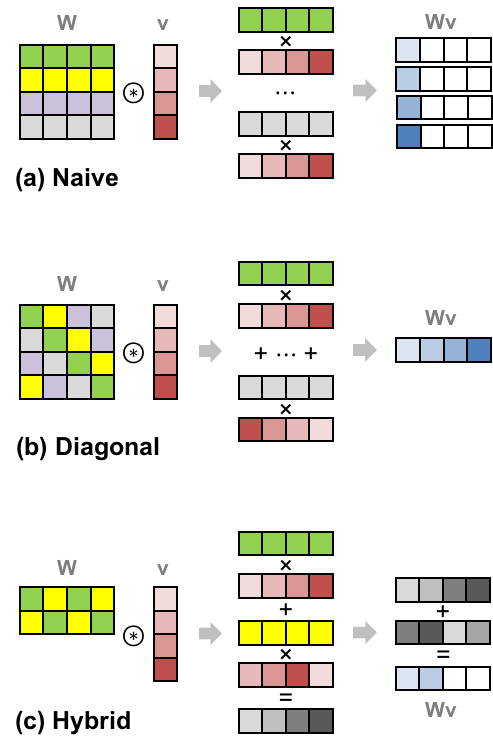
\includegraphics[width=0.4\linewidth]{figures/matrix-vector-multiplication-techniques.png}
  \caption[Image source: \cite{2018-gazelle}]{Different techniques to compute a dot product between a matrix and a vector,
    each having their up- and downsides.}
\end{figure}

\subsection{Adapting to non-square matrices}
The weight matrices in the given classification setting
are by no means square, on the contrary their output dimension tends
to be much lower than the input dimension as the goal is to reduce it from
$28^2 = 784$ to $10$ overall.

However, that also means one cannot directly apply the diagonal method
as described in the proceedings above.
This 'flaw' can be mitigated by a simple zero-padding approach
in order to make the matrix square, filling in zeros until
the lower dimension reaches the higher one.

\section{Polynomial Evaluation}
From the implementation perspective, there are three properties to watch out for when
working with SEAL ciphertexts:

\begin{enumerate}
  \item Scale (retrieved using \cpp{x.scale()})
        \begin{quote}
          Scale has nothing to do with noise. "Scale out of bounds" can appear even if noise is extremely low. Although repeated multiplication of a ciphertext by a plaintext will slowly increase the noise, it is not the reason why you see "scale out of bounds".
          "Scale out of bounds" error specifically means that the scale of a ciphertext or plaintext is larger than the product of all elements in coeff\_modulus. If you perform multiplications without rescaling, you can quickly see this error. The more rescaling you perform, the less elements will be left in coeff\_modulus. Even if you managed to have the same scale in a ciphertext after every multiplication and rescale, eventually the coeff\_modulus can be too small to accommodate another multiplication.
        \end{quote}
        % https://github.com/microsoft/SEAL/issues/182#issuecomment-646234787

        Can be adjusted with: \cpp{evaluator.rescale_inplace()}
  \item Encryption Parameters (retrieved using \cpp{x.parms_id()}) \\
        Can be adjusted with: \cpp{evaluator.mod_switch_to_inplace()}
  \item Ciphertext Size (retrieved using \cpp{x.size()}) \\
        Can be adjusted with: \cpp{evaluator.relinearize_inplace()}
\end{enumerate}

\paragraph{Multiplication}
Each time one multiplies two ciphertexts, the scales multiply (logarithmically, they add up, i.e. the bits are added together).
The chain index reduces by 1. The chain index of an encoded ciphertext depends on the coeff moduli.
There must be enough bits remaining to perform the multiplication, namely log2(scale) bits.

\paragraph{Addition}
The scales must be the same, but luckily they will not change.

\section{Transparent Ciphertext}
\begin{quote}
  The problem is that you are subtracting a ciphertext from itself.
  This kind of operation results in a ciphertext that is identically zero;
  this is called a transparent ciphertext. Such a transparent ciphertext
  is not considered to be valid because the ciphertext reveals its underlying plaintext to anyone who sees it,
  even if they don't have the secret key.
  By default SEAL throws an exception when such a situation is encountered to protect you from a problem you may not have noticed.
  If you truly know what you are doing and want to enable the creation of transparent ciphertexts,
  you can configure SEAL [...].
  \parencite{kim-laine-on-transparent-ciphertexts}
\end{quote}

% https://github.com/microsoft/SEAL/issues/276#issuecomment-777073477
'transparent ciphertexts (a.k.a. ciphertexts whose second polynomial is zero) are malformed and do not need the secret key to decrypt'
